\section{modelling}

\emph{Note: }We denote a Layer in a general meaning by 'physical layer' 
or 'MAC layer' and our concrete C++ classes by \h{\bp} or \h{\bm}.

\subsection{overview}

Here we present the design- and interface details of the OMNeT-module 
\h{\bp} to meet the requirement specification. That includes:

\begin{enumerate}
 \item internal class diagram of \h{\bp} and relation to \h{\bm}
 \item interface description for all involved C++ classes
 \item flow charts for reception of MacPacket from upper layer and 
 AirFrame from the channel
 \item some detailed flow charts for important sub processes
\end{enumerate}


\subsection{classgraph}

We start with the classgraph for the OMNeT-module \h{\bp} that shows 
its C++ classes, relations to other OMNeT-modules (especially \h{\bm})
and the OMNeT-messages sent between them.

The \h{\bp} holds a list\req{analogueMulti} of AnalogueModels and a pointer to a
Decider. Thus the AnalogueModel and the Decider are submodules of \h{\bp}. This
way one is able to change\req{analogueExtensible}\req{deciderExtensible} and
replace\req{analogueIndependent}\req{deciderIndependent} them independently from
the \h{\bp}.

\begin{figure}[H]
 \centering
 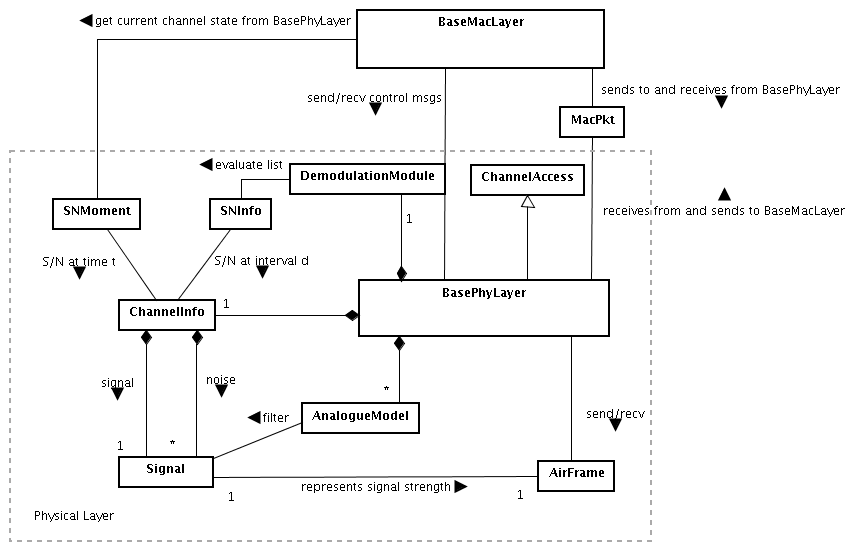
\includegraphics[width = \textwidth]{modelling/class_diagram.png}
 \caption{class graph}
 \label{fig: classgraph}
\end{figure}


\subsection{The \h{\bp} interface}

In this section we focus on how one is able to communicate with the 
\h{\bp}, i.e. especially the \h{\bm} which is connected to the \h{\bp}
in three ways:

\begin{enumerate}
 \item OMNeT-channel for data messages
 \item OMNeT-channel for control messages
 \item a reference to \h{\bp}.
\end{enumerate} 

The data channel is used to send and receive\req{packetFromMac} MacPkts to and
from the \h{\bp}.

The control channel is used by the \h{\bp} to inform the \h{\bm} about
certain events\req{provactive}, like the TX\_OVER\req{txover} message 
which indicates the end of a sending transmission.

The reference provides a passive way\req{provpassive} for the  \h{\bm} to  get
information about the current channel state\req{channelstate} and to
get\req{currentmode} and set\req{switchmode} the current radiostate (RX, TX,
SLEEP).
Switching times\req{switchtimes} from one radio state to another are controlled
internally by a state machine. \saf{mode state machine}.


\begin{figure}[H]
 \centering
 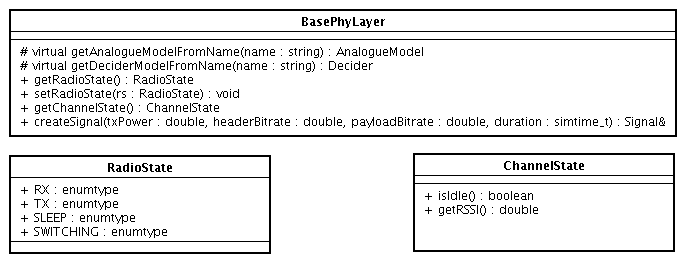
\includegraphics[width = \textwidth]{modelling/BasePhyLayer_members.png}
 \caption{BasePhyLayer interface}
 \label{fig: BasePhyLayer interface}
\end{figure}



\subsection{AnalogueModel}
%\label{AM and Signal}

%The Signal is designed one-dimensional (power-over-time) by default with a
%specified time point for start and end of the Signal. The owner is able
%to add and request values at a specific time point\req{sendInfoTXPower}.
%The Method getTimeIterator() returns an appropriate SignalTimeIterator needed
%for applying AnalogueModels to the Signal.

%\begin{quote}
%\emph{NOTE: Anyone who subclasses Signal should make shure to have a properly
%working SignalTimeIterator (subclassed) for it. The SignalTimeIterator should
%always iterate over every time stamp in each dimension. This way simple
%AnalogueModels will be able to filter the Signal independent from its
%dimension.}
%\end{quote}

%Further the Signal is set the packets bitrate over time\req{sendInfoBitrate}, 
%the Move of the Host\req{sendInfoMove}, the size of the
%packet\req{sendInfoSize} and the channel dimensions\req{sendInfoChannel} by
%\h{\bp}.
%
%\emph{See also \ref{AirFrame and Signal}.}

The AnalogueModel is at least able to filter the basic, one-dimensional Signal
from a start point to an end point in time.\\

Information how it works on a more complex multi-dimensional Signal are
explained at section \ref{sec:signaldetail}.
 
\begin{figure}[H]
 \centering
 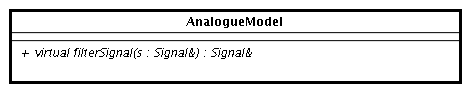
\includegraphics[width = \textwidth]{modelling/AnalogueModel_members.png}
 \caption{analogue model interface}
 \label{fig: analogue model interface}
\end{figure}
%
%The AnalogueModel offers functionality to filter a referenced
%signal\req{analogueFilter} in a specified interval\req{rcvFilterSignals} (e.g.
%preamble\req{rcvFilterPreamble}) or at a single point in time.

%Three basic AnalogueModel classes are foreseen to be plugged into Phy-Layer to
%simulate pathloss\req{analogueSimPathloss}, shadowing\req{analogueSimShadowing}
%and fading\req{analogueSimFading}.\\
%\h{\bp} is designed to apply an arbitrary number of AnalogueModels to a Signal.

% \begin{figure}[H]
%  \centering
%  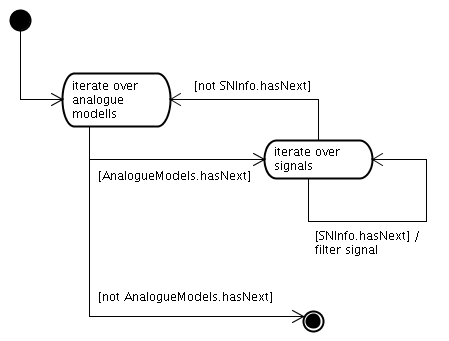
\includegraphics[width =
%0.8\textwidth]{modelling/apply_analogue_modells_detail.png}%[width=300pt]
%  \caption{application of analogue models}
%  \label{fig: application analogue models}
% \end{figure}



\subsection{ChannelInfo}

ChannelInfo keeps track of all AirFrames on the channel. It does not
differentiate between \textit{signal} and \textit{noise}. \h{\bp} is able to
add and remove references to certain AirFrames to and from ChannelInfo.\\
ChannelInfo can return a vector of Signals (references) that intersect with a
given time interval.\\
SNInfo is created by \h{\bp} when a packet arrives to collect all signals from
the channel that intersect with the reception time interval of the packet.

\begin{figure}[H]
 \centering
 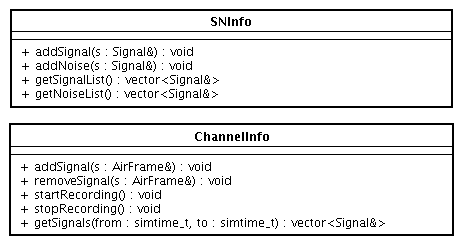
\includegraphics[width = \textwidth]{modelling/ChannelInfo_members.png}
 \caption{channel details}
 \label{fig: channel details}
\end{figure}




\subsection{Decider and SNInfo}
\label{decider}

The Decider has two tasks:
\begin{enumerate}
	\item It decides whether we are able to receive a certain packet as
\textit{signal}, otherwise the packet will be considered
\textit{noise}.\req{rcvClassify} The moment the AirFrame arrives, the Decider is
asked for a time interval after that it wants to be handed the SNInfo again to
make the decision.
	\item When a packet has been received and is not \textit{noise} the
Decider evaluates the SNInfo for that Signal and returns a DeciderResult that
only contains if the packet was received correct or not correct by
default\req{rcvIsCorrect}.
\end{enumerate}

A Decider that gives a richer DeciderResult (e.g. bitwise
errors\req{deciderBitwise}) must be subclassed and implemented by the user.

\begin{figure}[H]
 \centering
 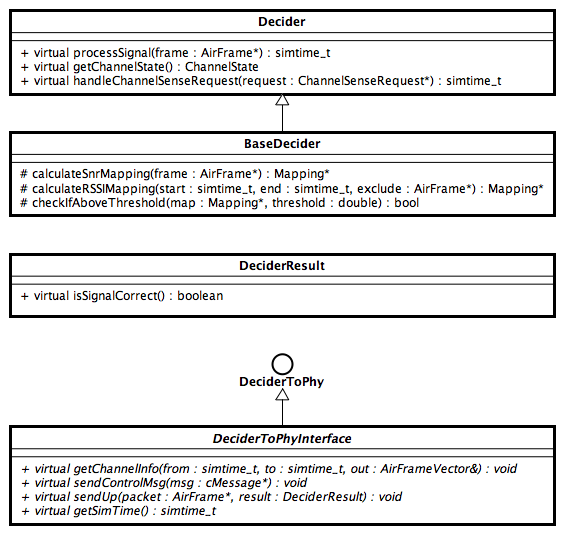
\includegraphics[width = \textwidth]{modelling/DeciderModule_members.png}
 \caption{Decider interface}
 \label{fig: Decider interface}
\end{figure}


\subsection{The one-dimensional Signal and AirFrame}
\label{AirFrame and Signal}

AirFrame and Signal are both initialized by \h{\bp} with information from
MacToPhyControlInfo.
It is shown below how nessecary information for sending/receiving is
distributed.\\

Here we focus on the basic, one-dimensional (time) Signal that stores entries
for TX Power and attenuation over time. There are fix entries for header and
payload bitrate. These assumptions are considered to cover most cases.
It is possible to obtain a time iterator for this Signal to have access to
entries at specific time points.
Further Signal stores the Move (move pattern of the sending host), the packets
header length, the start time and length of the Signal.\\

\emph{Note: The multi-dimensional Signal is an instance of the same class but
has more functionality. It is described in detail in a separate section.}\\

\h{\bp} calculates duration\req{sendInfoDuration} and preamble
duration\req{sendInfoPreambleDuration} of the packet and adds it to the
AirFrame. 
To be able to control the sending process\req{sendControl} of another AirFrame
every AirFrame has a unique id and a specific type which secifies if this is a
normal AirFrame or a control-AirFrame.


\begin{figure}[H]
 \centering
 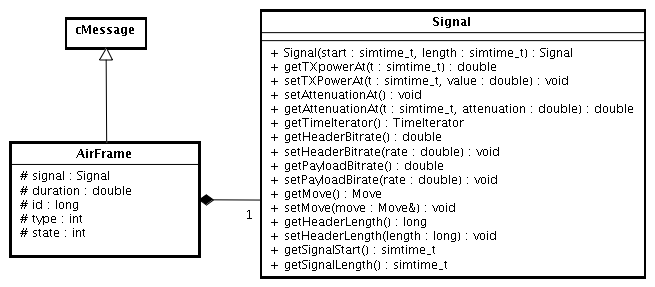
\includegraphics[width = \textwidth]{modelling/AirFrame_members.png}
 \caption{member arrangement in AirFrame and Signal}
 \label{fig:memberAirFrame}
\end{figure}
\newpage
